\subsection{Query Candidate Ranking}
\label{sec:ranking}


It is possible that multiple SQL queries satisfying
the given input-output examples will be returned.
This may adversely impact end-users who want to
write simple query tasks but now may require
to provide more bits for disambiguation of their intent (which
manifests in the need to provide more examples and more rounds
of interaction). To alleviate this problem, we employ
the Occam's razor principle, which states that the
simplest explanation is usually the correct one, to
rank the more likely queries higher in the output list.
We define a comparison scheme between different
SQL queries by defining a partial order between them. Some of
these choices are subjective, but have been observed to work well.

A SQL query is simpler than another one if it uses
smaller number of query conditions (including \CodeIn{having}
and \CodeIn{order by}) or the expressions
in each query condition are pairwise simpler.
Simpler query conditions suggests the extraction logics
are more common and general.

In our implementation, \ourtool computes a cost for each
query, and prefers queries with lower costs. The cost
for a SQL query is computing by summarizing the text length
of each query condition used. Figure~\ref{fig:rank} shows an example.


\begin{figure}[t]
\centering
 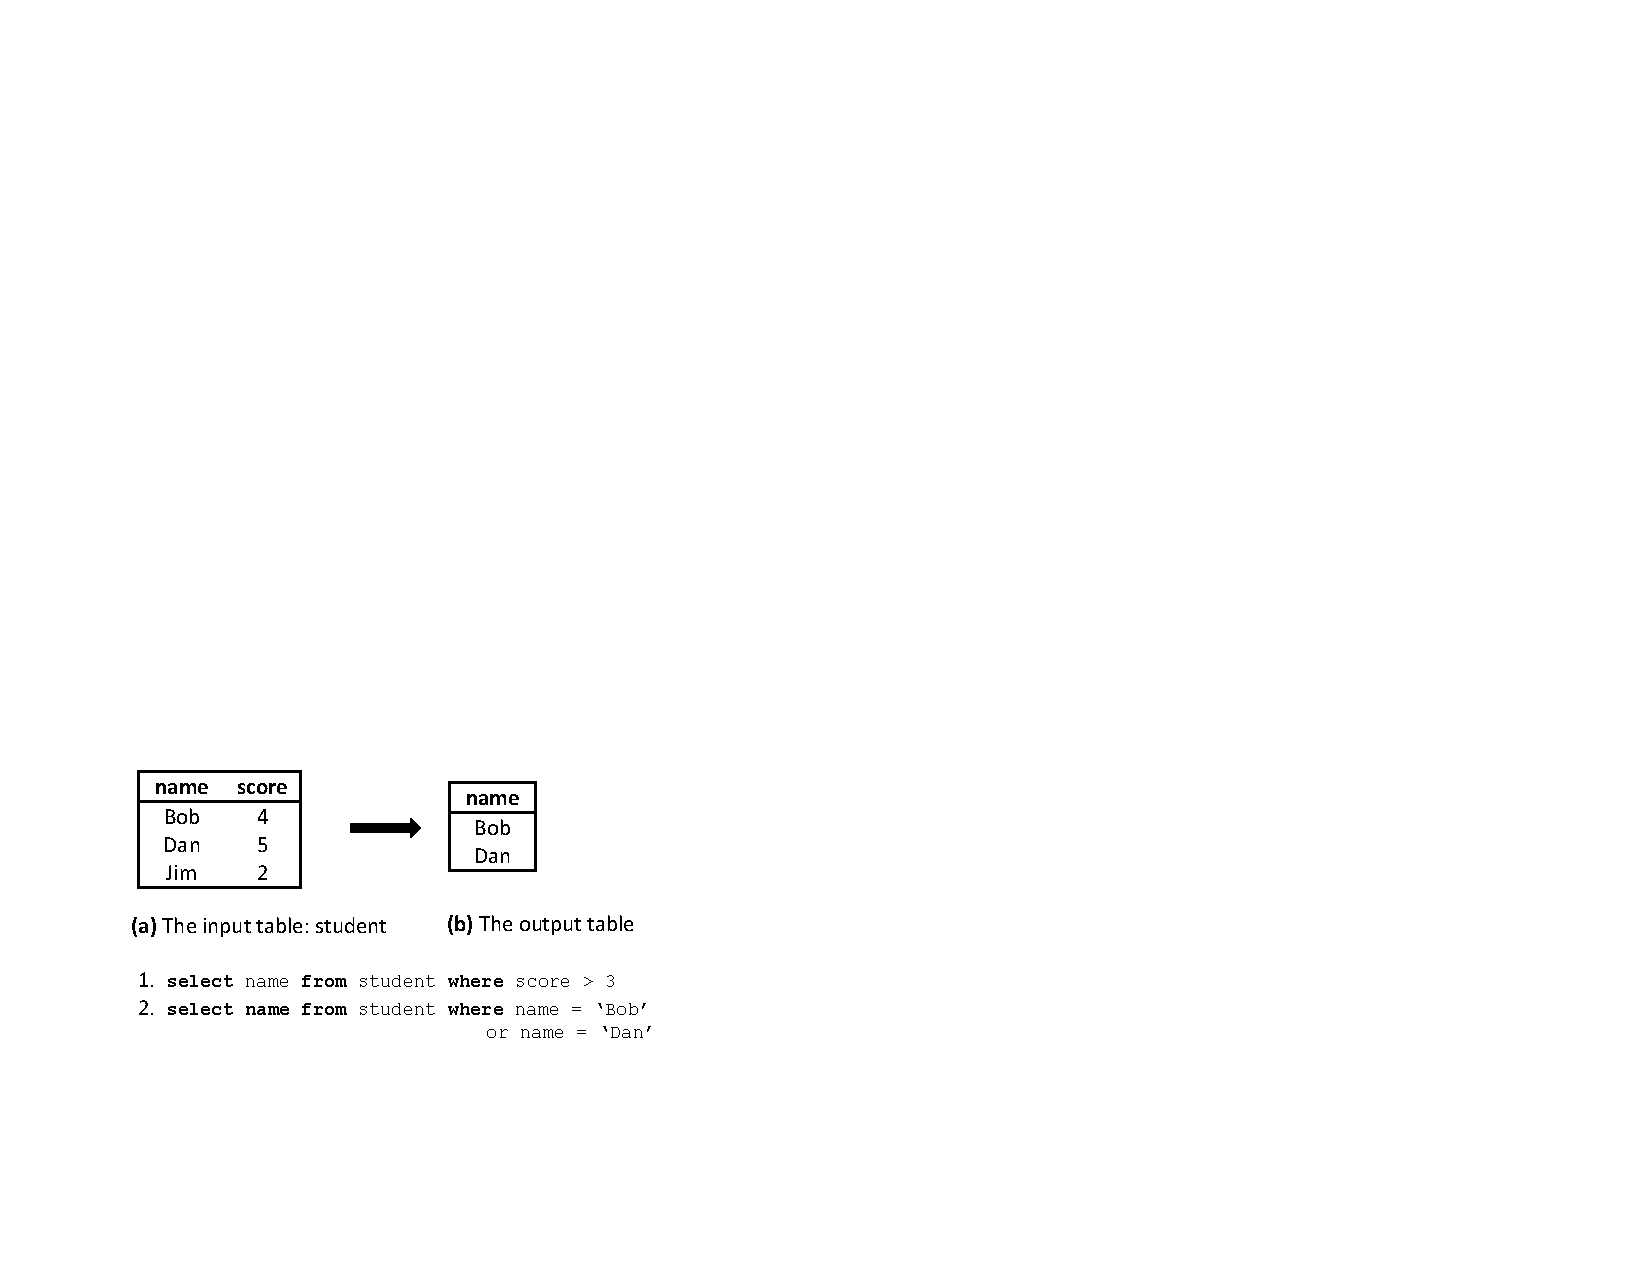
\includegraphics[scale=0.80]{rankexample}
 \vspace{-3mm}
\Caption{{\label{fig:rank} Illustration of \ourtool's
query candidate ranking strategy. \ourtool produces two
queries for the given input-output examples. Based on
our heuristic (Section~\ref{sec:ranking}), the first query
differs from the second query by using simpler conditions,
and thus ranks higher (and is less likely to overfit the
given examples).
}}
\end{figure}

